\documentclass[a4paper,utf,ngerman]{article}
\usepackage{babel}
\usepackage{inputenc}
\usepackage{graphicx}
\usepackage{fancyhdr}
%
\fancypagestyle{ktsipage}{%
  \fancyhf{} % clear all header and footer fields
  % l: left, r: right, o:odd, e: even
  \fancyhead[lo]{Software-Engineering}
  \fancyhead[ro]{UML}
%  \fancyhead[le,ro]{}
%  \fancyfoot[ro]{\small\sf Oktober 2008}
  \fancyfoot[lo,re]{\small R. Tanner}
}
%
\pagestyle{ktsipage}
%
\begin{document}
\section*{Projekt StopWatch}
Es soll eine Stoppuhr implementiert werden, die 
die folgenden Eigenschaften aufweist:
\begin{enumerate}
  \item Die Stoppuhr kann ein- und ausgeschaltet werden.
  \item Die Stoppuhr kann gestartet und gestoppt werden. Nach dem
  Stopp wird die abgelaufene Zeit zwischen Start und Stopp angezeigt.
  \item Nach dem Start kann eine Zwischenzeit angezeigt werden.
   Die Uhr läuft im Hintergrund weiter. Nun kann entweder die
   Anzeige von der Zwischenzeit auf die Anzeige 
   der aktuell abgelaufenen Gesamtzeit gewechselt werden
   oder die im Hintergrund laufende Uhr kann angehalten werden,
   ohne dass sich die Anzeige ändert. Im letzten Fall
   wird nach einem weiterem Knopfdruck die vergangene 
  Gesamtzeit angezeigt.
  \item Die zwischen Start und Stopp vergangene Zeit kann
   bei gestoppter Uhr und Anzeige der vergangenen Gesamtzeit
   auf Null zurückgesetzt werden.
 \item Die Uhr besitzt zwei Druckknöpfe, die nicht gleichzeitig
  gedrückt werden können, und eine vierziffrige Anzeige.
\end{enumerate}
\begin{figure}[H]
\centering
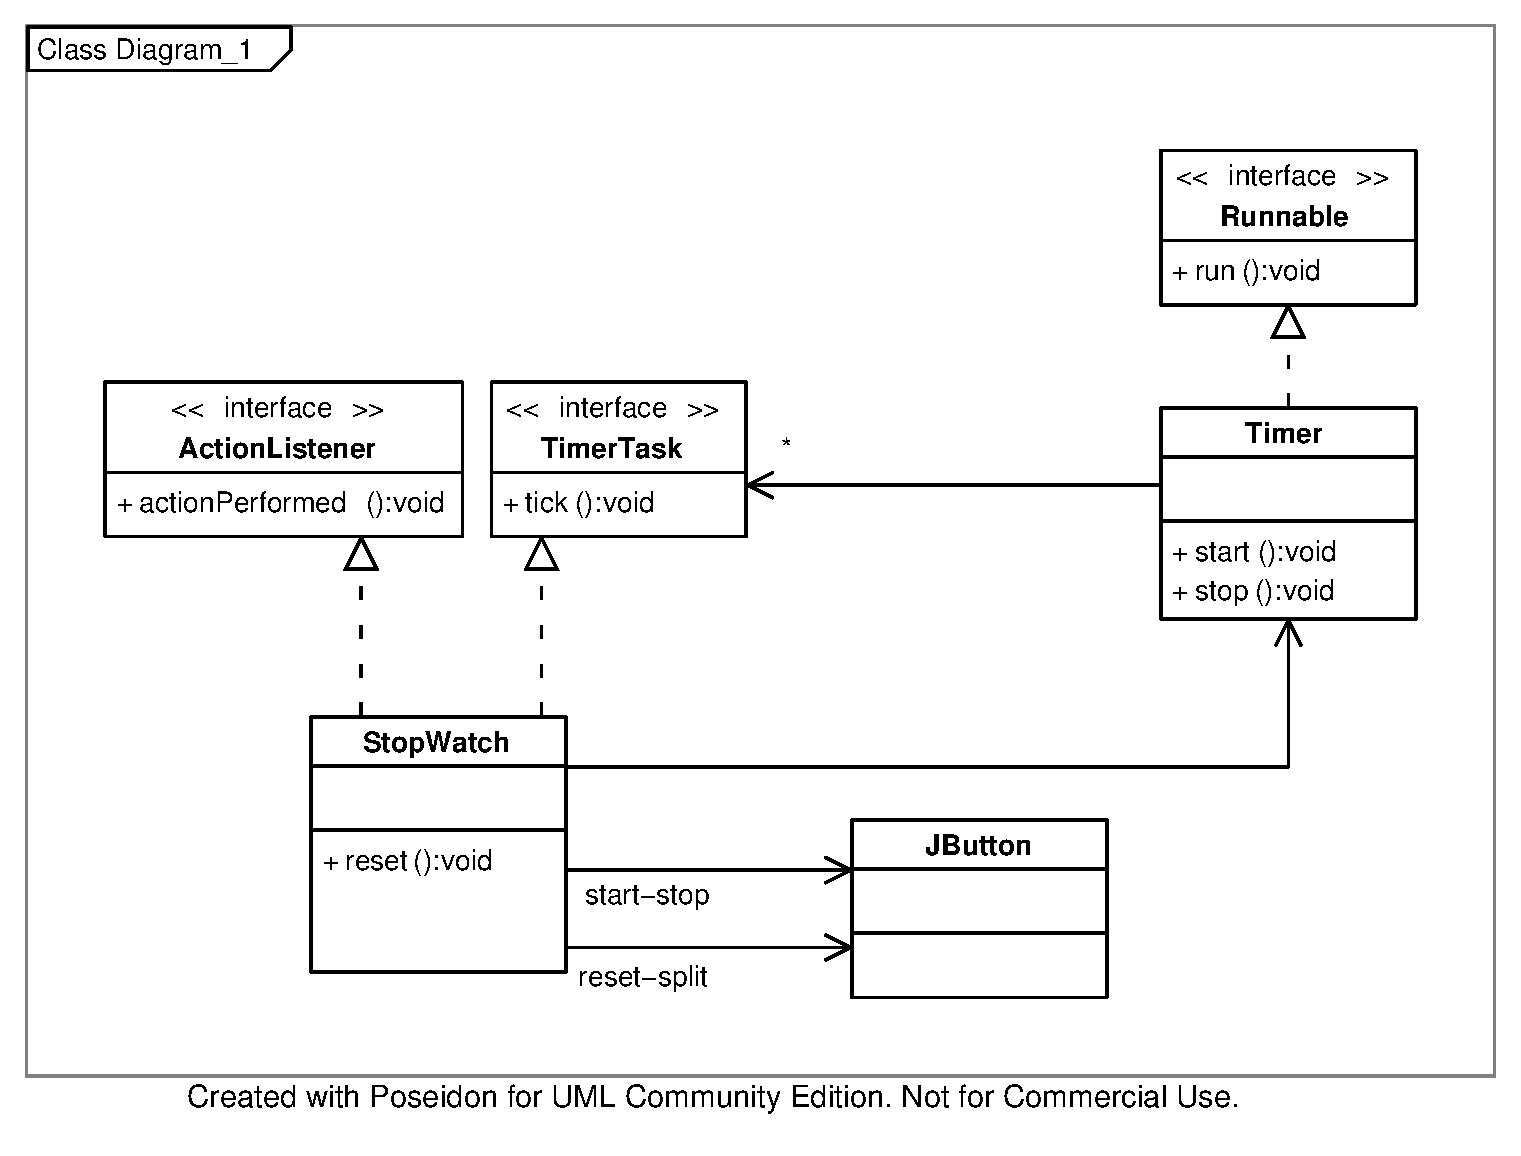
\includegraphics[trim=20 60 50 40,width=\linewidth,clip=true]{ClassDiagram}
\caption{Klassendiagramm}
\end{figure}
\begin{figure}[H]
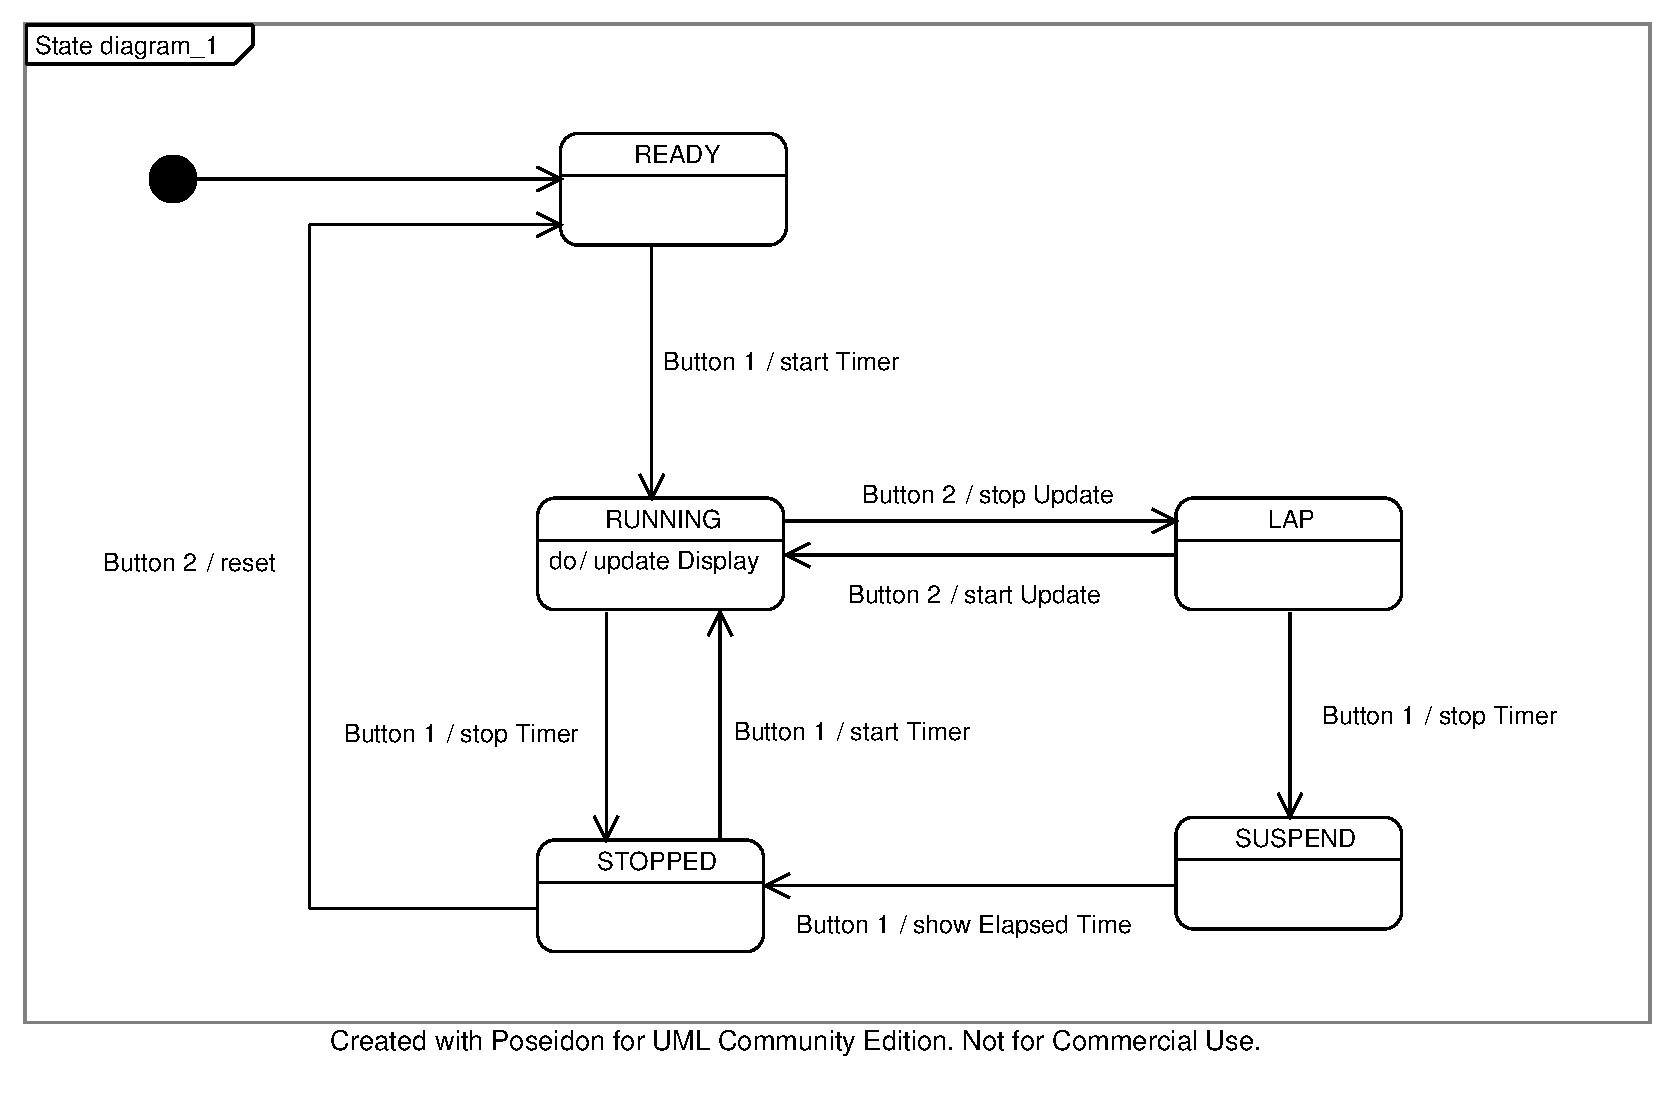
\includegraphics[trim=20 40 60 40,width=\linewidth,clip=true]{Statediagram}
\caption{Zustandsdiagramm}
\end{figure}
\end{document}
